\documentclass[shadesubsections,compress,14pt,mathserif]{beamer}
\usepackage[danish]{babel}	
\usepackage{tikz}
\usetikzlibrary{shapes, positioning}
\usenavigationsymbolstemplate{}
\usepackage{pgfplots}
\usepackage[absolute,overlay]{textpos}
\usepackage{amsthm}
%\usepackage[T1]{fontenc}
%\usepackage{fourier}
% Dokumentets sprog
%\usepackage{mathtools}
%\usepackage{pxfonts}
\usepackage{eulervm}
% Class options include: notes, notesonly, handout, trans,
%                        hidesubsections, shadesubsections,
%                        inrow, blue, red, grey, brown

% Theme for beamer presentation.
%\usepackage{beamertheme} 
% Other themes include: beamerthemebars, beamerthemelined, 
%                       beamerthemetree, beamerthemetreebars  
 \newcommand{\prot}{\mathbf{P}}
\newcommand{\adv}{\ensuremath{\mathcal A}}
\newcommand{\aggdeg}[1]{\mathfrak{d}(#1)}
\renewcommand{\deg}{\mathrm{deg}}
\newcommand{\xor}{\ensuremath{\oplus}}
\newcommand{\plonk}{\ensuremath{\mathcal{P} \mathfrak{lon}\mathcal{K}}}
\newcommand{\F}{\ensuremath{\mathbb F}}
\newcommand{\set}[1]{\ensuremath{\left\{#1\right\}}}
\newcommand{\sett}[2]{\ensuremath{\left\{#1\right\}_{#2}}}
\newcommand{\enc}[1]{\ensuremath{\left[#1\right ]}}
\newcommand{\cm}{\ensuremath{\mathsf{cm}}}
\newcommand{\open}[1]{\ensuremath{\mathsf{open}(#1)}}
\newcommand{\verify}[1]{\ensuremath{\mathsf{verify}(#1)}}
\newcommand{\defeq}{\ensuremath{:=}}
\newcommand{\helper}{\ensuremath{\mathcal{H}}}
\newcommand{\ver}{\ensuremath{\mathcal{V}}}
\newcommand{\prv}{\ensuremath{\mathcal{P}}}
 \newcommand{\polysofdeg}[1]{\F_{< #1}[X]}
 \newcommand{\polys}{\F[X]}
\newcommand{\acc}{{\mathbf{acc}}}
\newcommand{\ideal}{\mathbf{I}}
\newcommand{\gen}{\alpha}
\newcommand{\plookup}{\mathsf{plookup}}
\newcommand{\nl}{\\ \pause \vspace{0.2in}}
\newcommand{\nlnp}{\\ \vspace{0.2in}}
\newcommand{\stitle}[1]{{\large{\textcolor{purple}{\emph{#1}}}}}
\newcommand{\roots}{\ensuremath\textrm{roots}}
\setbeamersize{text margin left=3mm,text margin right=3mm} 
\title{\large{Medfree is the new vegan, vioxx shenaningans and futarchy}}    % Enter your title between curly braces
\author{\small{Ariel Gabizon}\\                 % Enter your name between curly braces
\tt{\footnotesize{\textbf{Aztec - which doesn't necessarily endorse the following messages ;)} }}  }                                     
\begin{document}
\boldmath
% Creates title page of slide show using above information
\begin{frame}
\maketitle
\end{frame}



\begin{frame}
Like most restaurants have one or two vegetarian and vegan option, every community
should have a \emph{MedFree} option.\nl
\textbf{MedFree} - Participation does not require mandatory medical interventions, including invasive tests.\nl
\emph{A goal of this conference is to put such an option ``on the menu'' of the zero-knowledge community.}
\end{frame}

\begin{frame}
\large{\textcolor{purple}{\emph{The ``zero-knowledge'' community?...A community of people who don't know anything?}}}\nl

Zero-Knowledge proofs are a cryptographic tool an order of magnitude more powerful than encryption.\\
\vspace{0.2in}
\emph{``If encryption is a light switch, zk proofs are a dimmer''}\nl
\end{frame}
\begin{frame}
 First conceived in 1985, zk-proofs lived mainly in theory papers for 30 years.\nl
 In the last decade, they've become more practical, and a multititude of companies are writing zkp software.\nl
 \textcolor{blue}{Many consider zk-snarks, a type of zkp, \textbf{the} tool for blockchain privacy and scalability solutions. Hence, the zk community heavily overlaps with several blockchain communities like Ethereum.}
\end{frame}
\begin{frame}
\large{\textcolor{purple}{\emph{Why MedFree?}}}\nl
%  \smalltitle{Why MedFree?}
 Let's go back in history 20 years and talk about Vioxx (we're all sick of talking about covid, right?) \nl
 \textcolor{blue}{..but let's stop and talk about Theranos one sec..
 that story alway gave me a warm and fuzzy feeling..why?\nl}
 \textbf{The subtext:}This was a very extreme exception $\Rightarrow$ the system is fine!!
\end{frame}
\begin{frame}
 \stitle{Credits}
 \emph{Based on Chapter one of ``Sickening'' by John Abramson}\nl
Anecdotally, a notorious covid \textbf{pro}-vaxer.
\end{frame}
\begin{frame}
 \frametitle{Vioxx}
 \begin{itemize}
  \item Developed by Merck for arthritis; approved in 1999.
  \item Used by 25 million Americans.
  \item Last year on market - 2.5 Billion usd in revenue.\pause
  
  \item \textcolor{red}{Sept 2004 - taken off market after study showing it doubles risk of heart attack and stroke.}
  \item estimated deaths caused: 40,000 - 60,000  \emph{``..roughly the number of American soldiers who died in the Vietnam War''}.\pause
\item 2007 - Merck pays 4.85 Bil to settle civil suit of 27k plaintiffs claiming Vioxx caused their storke/heart attack.
\item 2011 - Merck pays another 1B to settle other allegations.
 \end{itemize}

\end{frame}
\begin{frame}
 \stitle{How it began:}\\
 NSAIDs (Ibuprofen,Naproxen,..)
 \begin{itemize}
  \item 
 Work by inhibiting an enzyme called Cyclooxygenase (COX). Results in reduction of pain, inflammation, fever.\nl
 \item But since COX protects the stomach lining, this inhibition can cause GI/stomach problems, at worst case a \emph{hole} in your colon (perforated ulcer).
 \end{itemize}

 
\end{frame}
\begin{frame}
 \stitle{The COX-2 hypothesis}
 Scientists discovered COX has two forms
 \begin{itemize}
  \item COX-1 protects lining of stomach.
  \item COX-2 leads to inflammation.\nl
 \end{itemize}
So let's develop drugs that only inhibit COX-2!\nl
\emph{The catch:} COX-1 and COX-2 balance each other in vascular system.COX-1 makes blood clots more likely, COX-2 opens blood vessels, makes them less likely.
\end{frame}
\begin{frame}
 \stitle{Side thought: Is modern drug therapy an 8 year-old debugging code?}\\
 $\vdots$\\
 \emph{100 lines of code}\\
 $\vdots$\\
\texttt{ i++;}\\
 $\vdots$\\
 \emph{100 lines of code\\}
 $\vdots$\\
\texttt{print(i);}\nlnp
 
 \emph{\textcolor{blue}{``Hmmm..the computer printed 5 when I wanted 4 so I'll delete that i++..''}}
\end{frame}
\begin{frame}
 \frametitle{The first Vioxx paper - Nov, 2000}
 \emph{The VIGOR study showed 4 times more heart attacks, and 25$\%$ higher all-cause mortality when
 using Vioxx vs a traditional NSAID (Naproxen).}
 \begin{figure}
  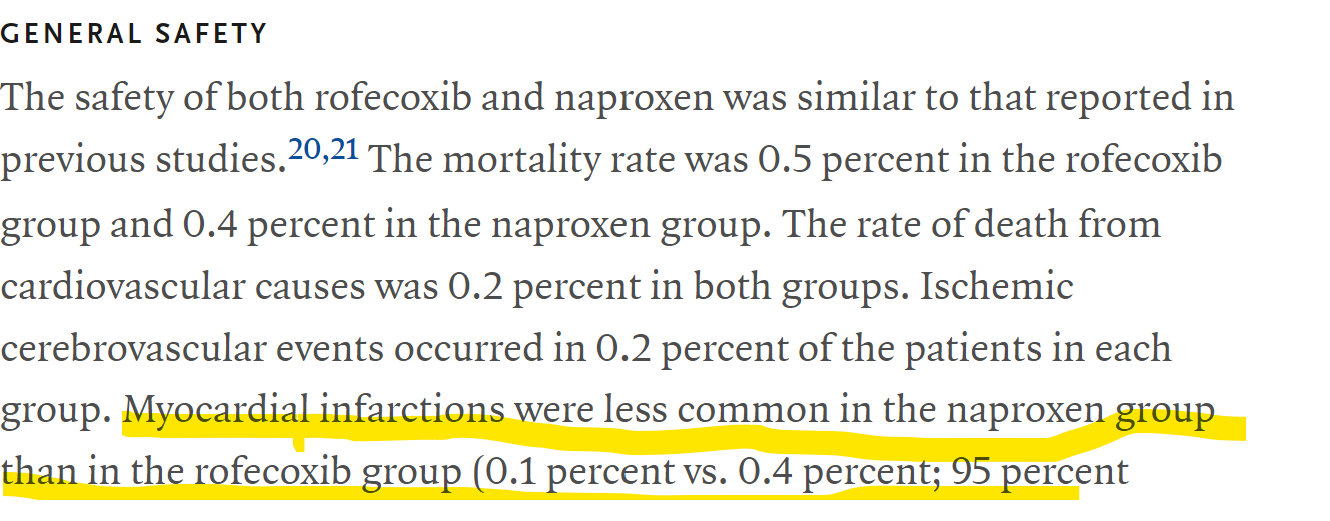
\includegraphics[width=300pt]{vioxxfirstsafety.png}
%   \caption{A boat.}
%   \label{fig:boat1}
\end{figure}
\end{frame}
\begin{frame}
 \stitle{Michael Jordan level moves - explaining away a 4X increase in heart attacks.}
 \begin{figure}
  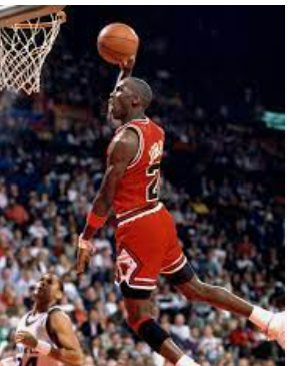
\includegraphics[width=30pt]{jordan.png}
%   \caption{A boat.}
%   \label{fig:boat1}
\end{figure}
\textcolor{brown}{4\% of participants where prone to heart attack, so ``met FDA criteria'' for use of Aspirin as protection..but couldn't take it during study. The statistical significance was only in that group:}
 \begin{figure}
  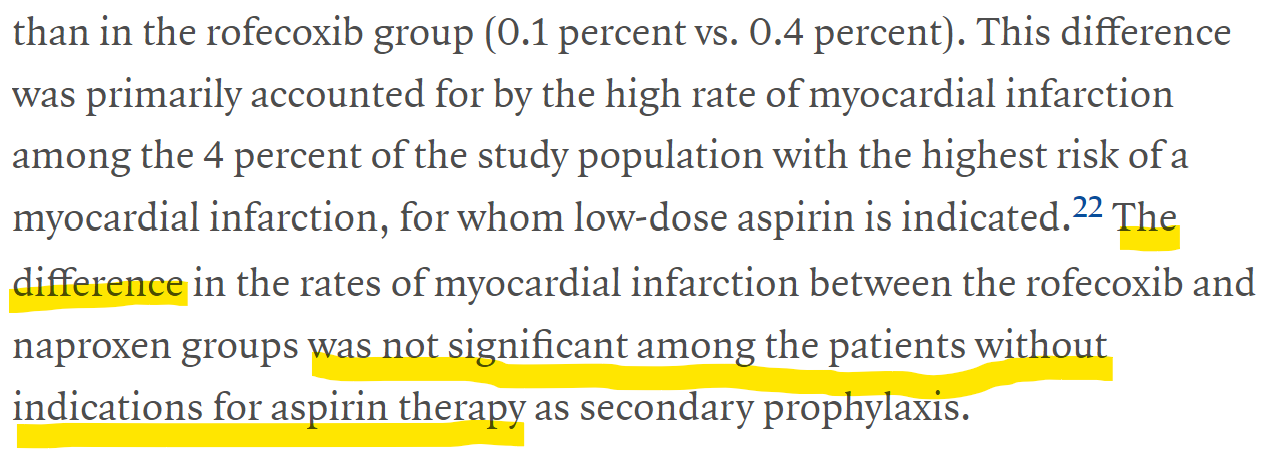
\includegraphics[height=90pt]{vioxxfirstsecondtxt.png}
\end{figure}\pause
{\tiny\emph{Remark: These were not people actually \textbf{taking} Aspirin - those were already excluded from the trial}}

 
\end{frame}
\begin{frame}
 \frametitle{Except that even that questionable logic was a flat out \textbf{lie}}\pause
%  https://www.nejm.org/doi/full/10.1056/NEJMe068054
 \begin{figure}
  \includegraphics[width=300pt]{3missing.png}
\end{figure}
 
 
 
\end{frame}
\begin{frame}
 \frametitle{Brought to you by Pfizer!..I mean Merck}
 \begin{figure}
  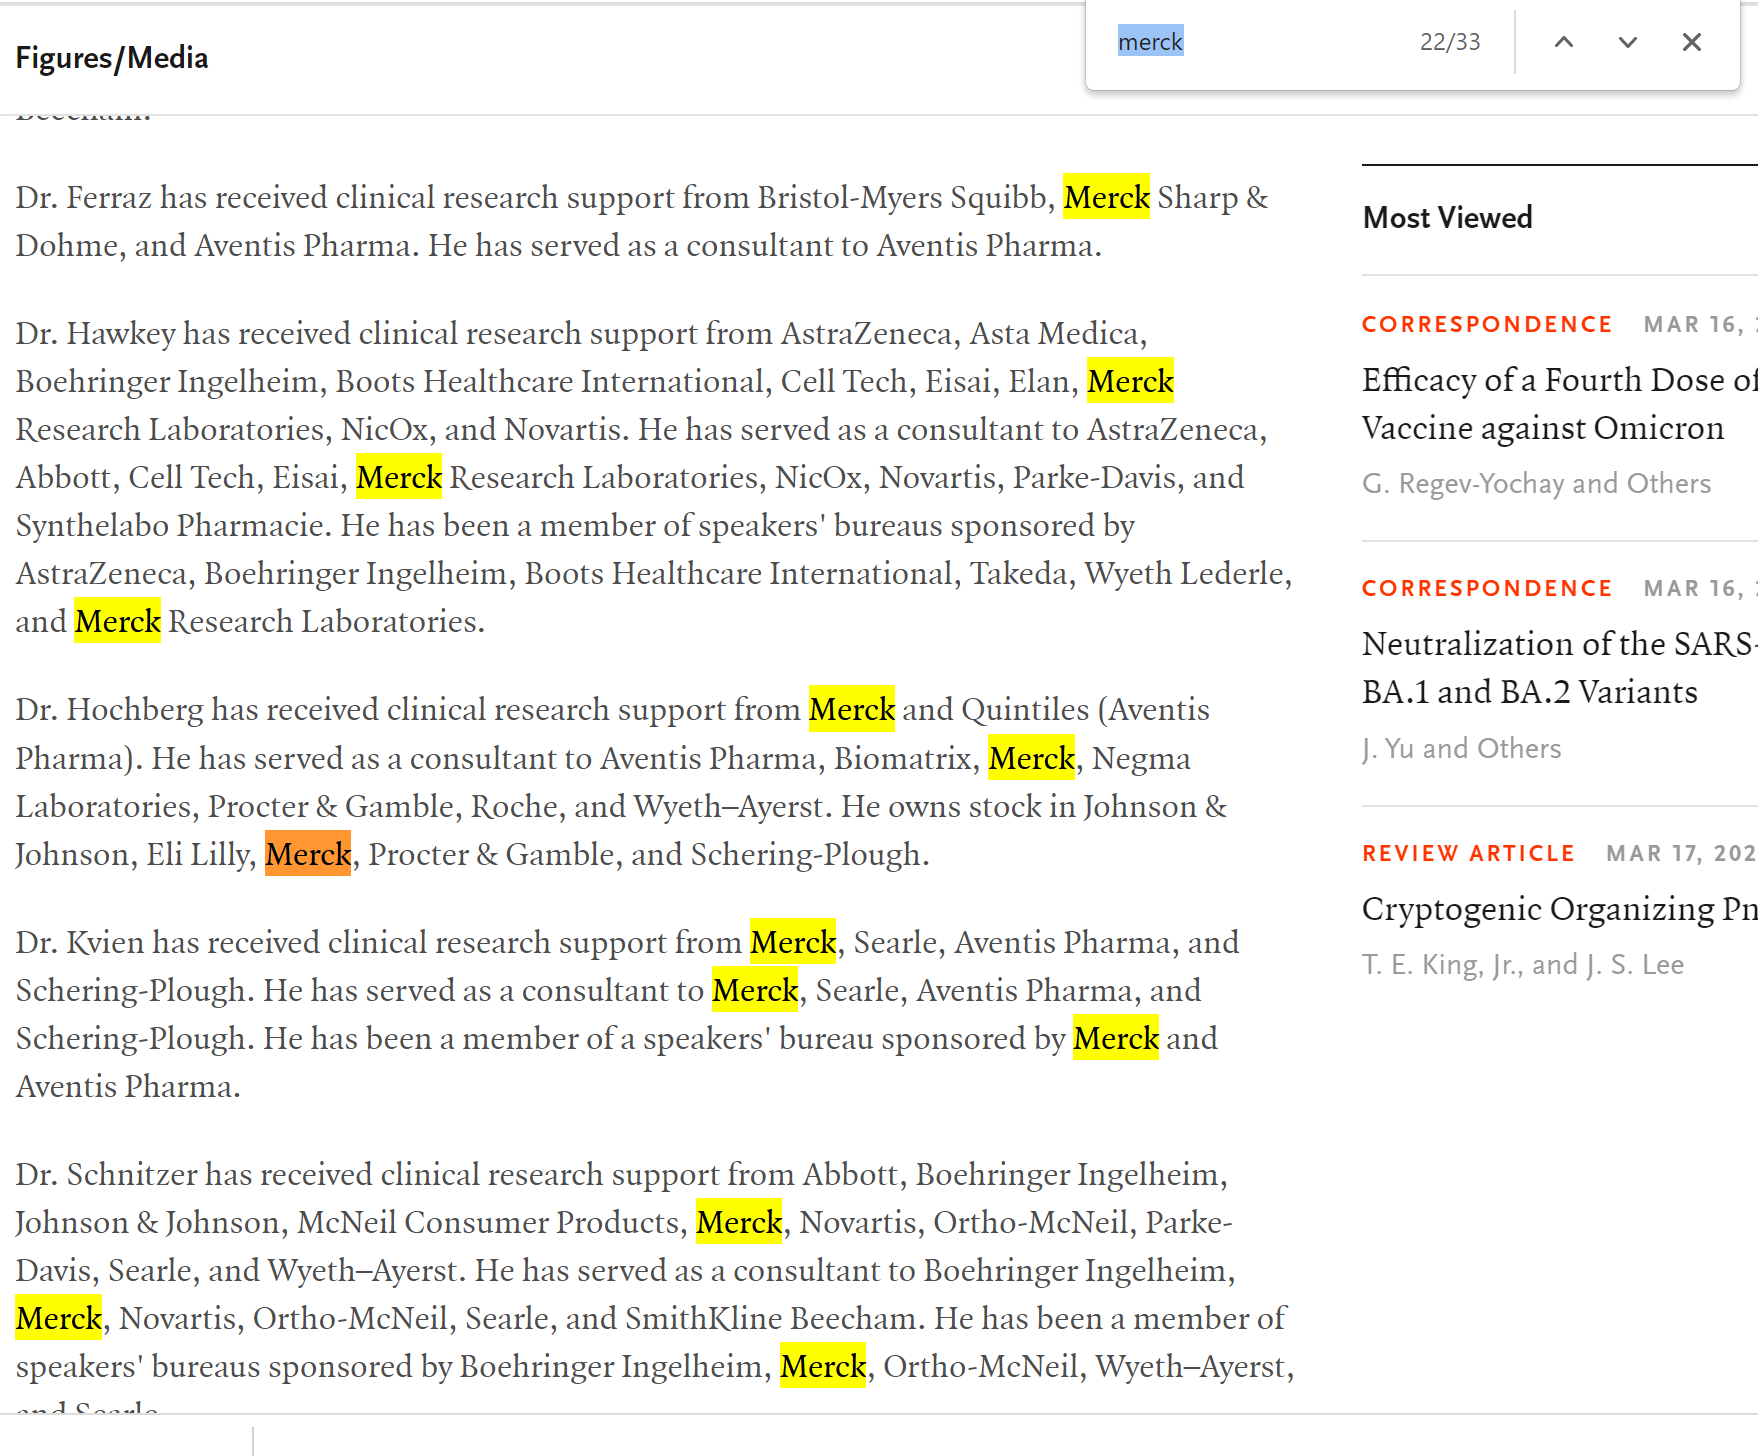
\includegraphics[width=300pt]{merck.png}
\end{figure}
 
\end{frame}
\begin{frame}
 \frametitle{The second paper in NEJM - Aug, 2001}
 \begin{figure}
  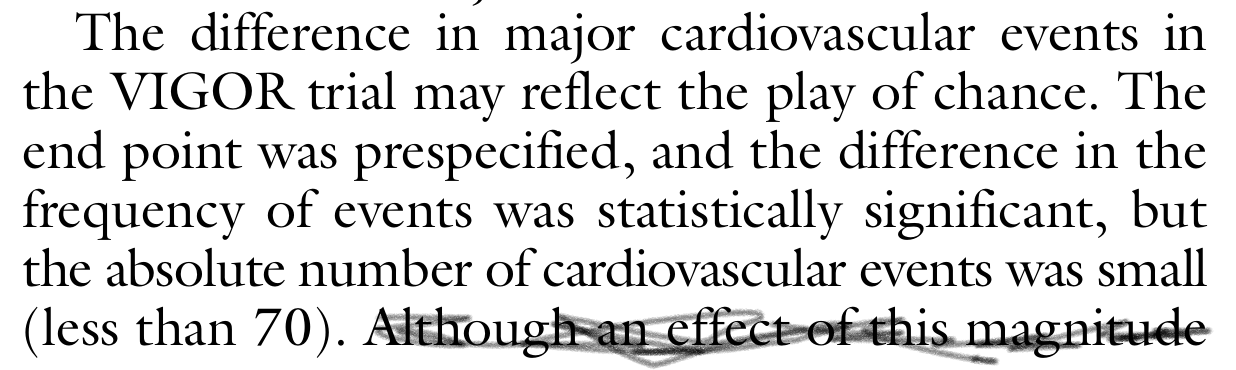
\includegraphics[width=300pt]{secondpaperquote.png}
\end{figure}
% total 53  GI events https://www.nejm.org/doi/full/10.1056/nejm200011233432103

%16 vs 37 in second row of table 4
 
\end{frame}
\begin{frame}
 \frametitle{Ad Laundering}
 Merck purchased 929,000 reprints of these articles from the NEJM for a price of between 697k to 836k usd, which it sent
 to doctors.
\end{frame}
\begin{frame}
 \frametitle{The information lag}
 \textbf{2001:} FDA warning to Merck to stop marketing Vioxx as safe.\nlnp
 \textbf{2004:} Stacey Palmer dies at 17; a healthy girl getting Vioxx for a headache from her doctor - samples he got from Merck.
 \end{frame}
\begin{frame}
 \emph{Now coming to covid..}\nl
 %Show Kratos animation
 %https://youtu.be/JmhZZOH6IZ4?t=63
The pharma moster has been turbo-charged with the power of government mandates.
\end{frame}
\begin{frame}
 Pfizer trial - the impressive part:
 %https://www.nejm.org/doi/suppl/10.1056/NEJMoa2110345/suppl_file/nejmoa2110345_appendix.pdf
 \begin{figure}
  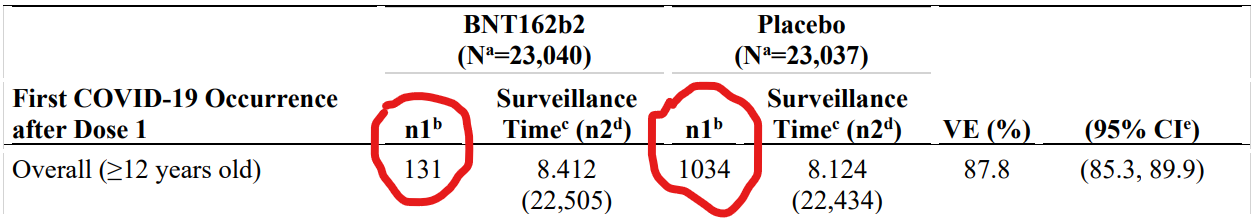
\includegraphics[width=200pt]{pfizergood1.png}
  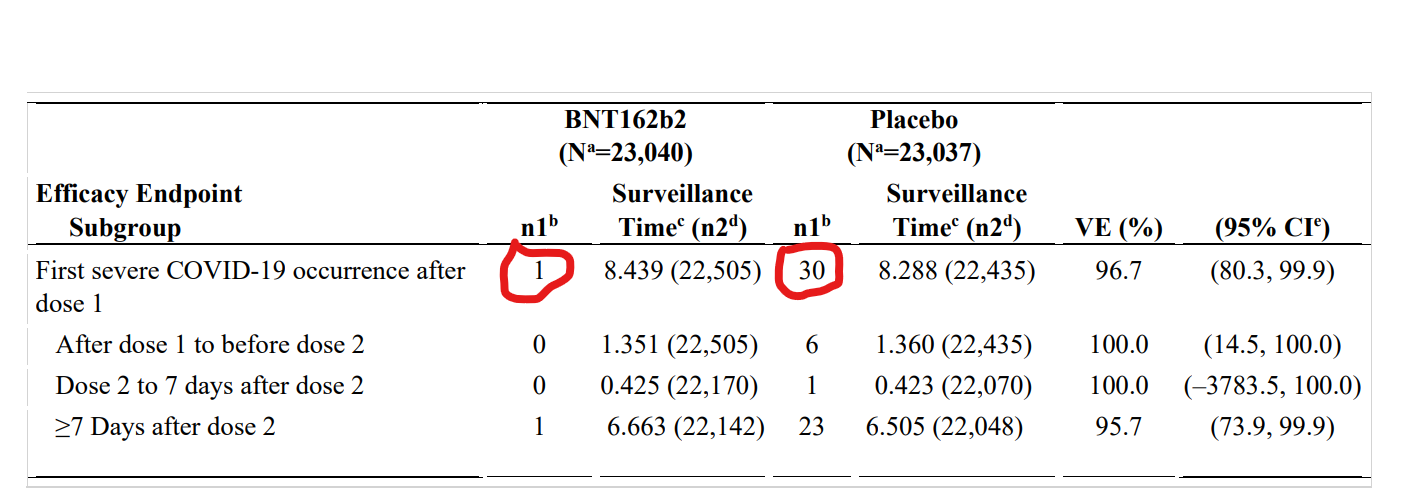
\includegraphics[width=200pt]{pfizergood2.png}
\end{figure}

\end{frame}

\begin{frame}
Pfizer trial all cause mortality after \textbf{early unblinding}:
 \begin{figure}
  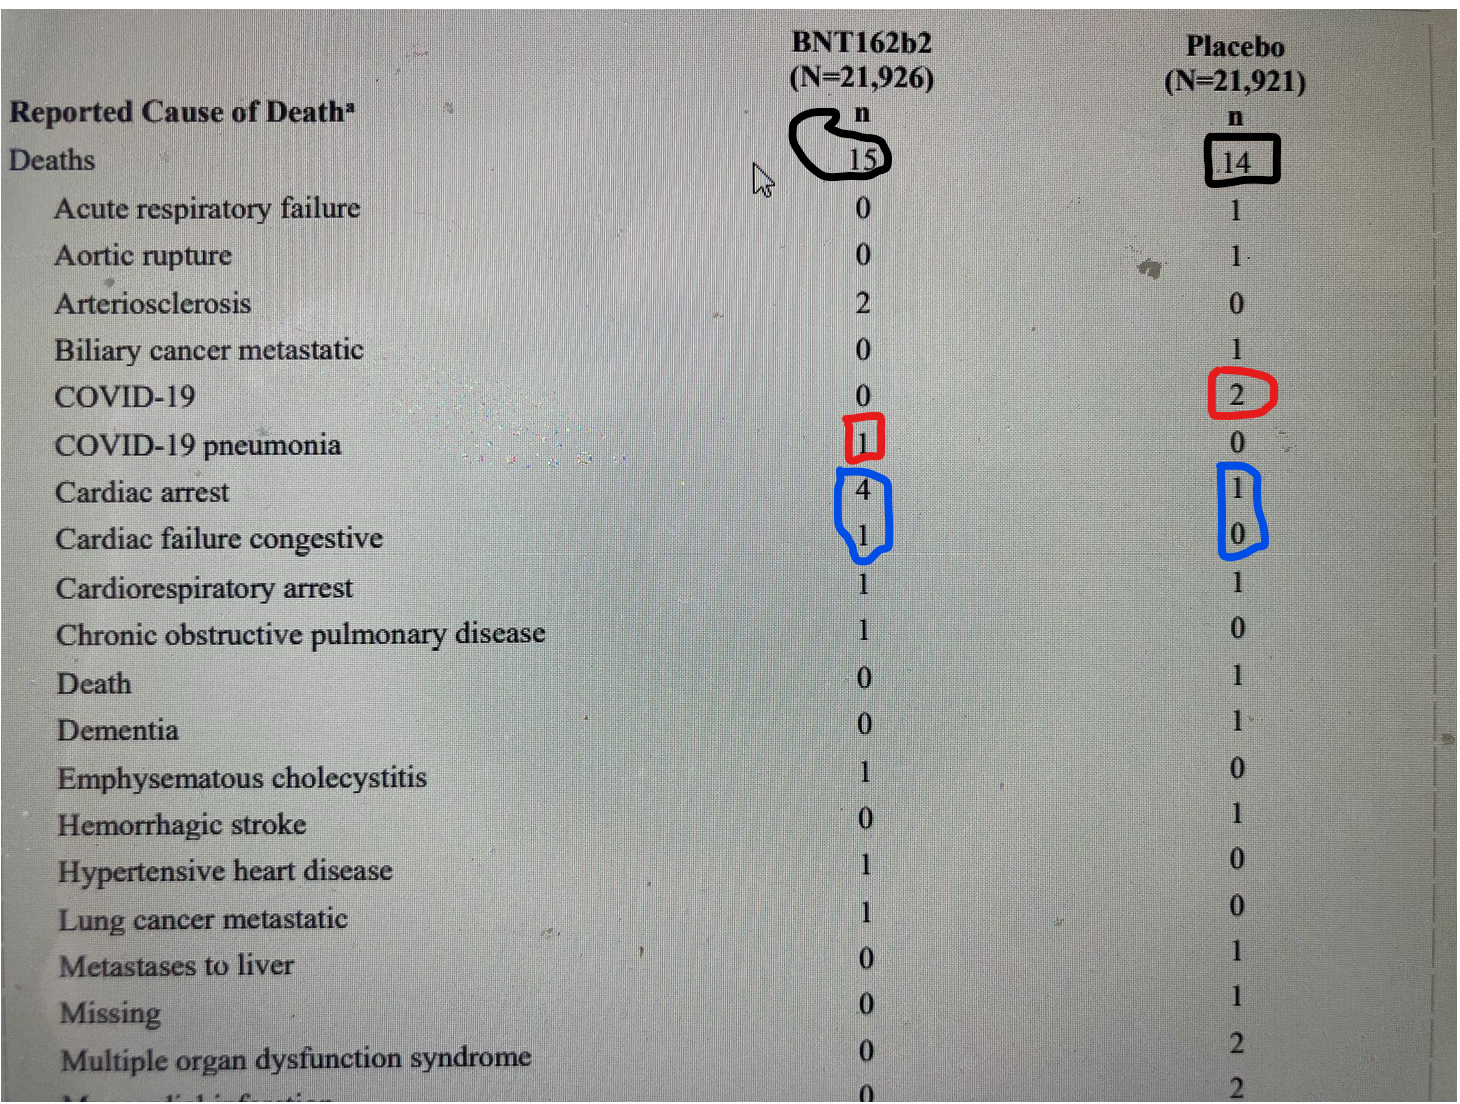
\includegraphics[width=300pt]{pfizerinitialallcausemortality.png}
\end{figure}

\end{frame}
\begin{frame}
 \stitle{Except that that those numbers turned out to be wrong}\\
 From  report on FDA site a few months later:
 \begin{figure}
  \includegraphics[width=300pt]{allcauseupdated.png}
\end{figure}
 
\end{frame}
\begin{frame}
 \stitle{Even my once beloved meditation school is now mandating vaccines and giving medical advice}\\
 \begin{figure}
  \includegraphics[width=300pt]{dhara.png}
\end{figure}
 
\end{frame}
\begin{frame}
\frametitle{A word about tests}
Are we going to use tests that exclude almost as many healthy people from events as sick?
 \begin{figure}
  \includegraphics[width=300pt]{antigenfalse.png}
%  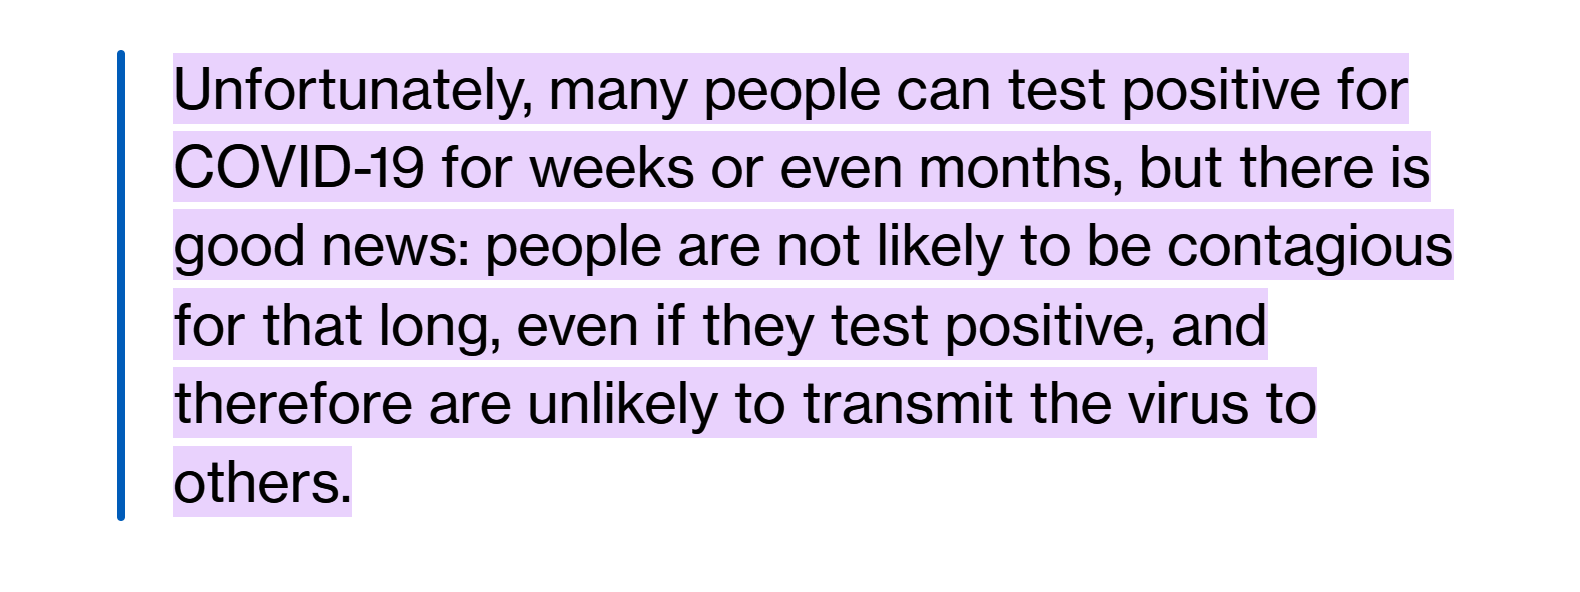
\includegraphics[width=300pt]{pcrfalsepos.png}
\end{figure}
 
\end{frame}
\begin{frame}
\stitle{In cryptographic terms - the prover and verifier got mixed up. Pharma company does the trial, and decides which
data to represent to journal reviewers - which questions to answer.}
\end{frame}
\begin{frame}
 \frametitle{Little Chariot vs Big Chariot}
  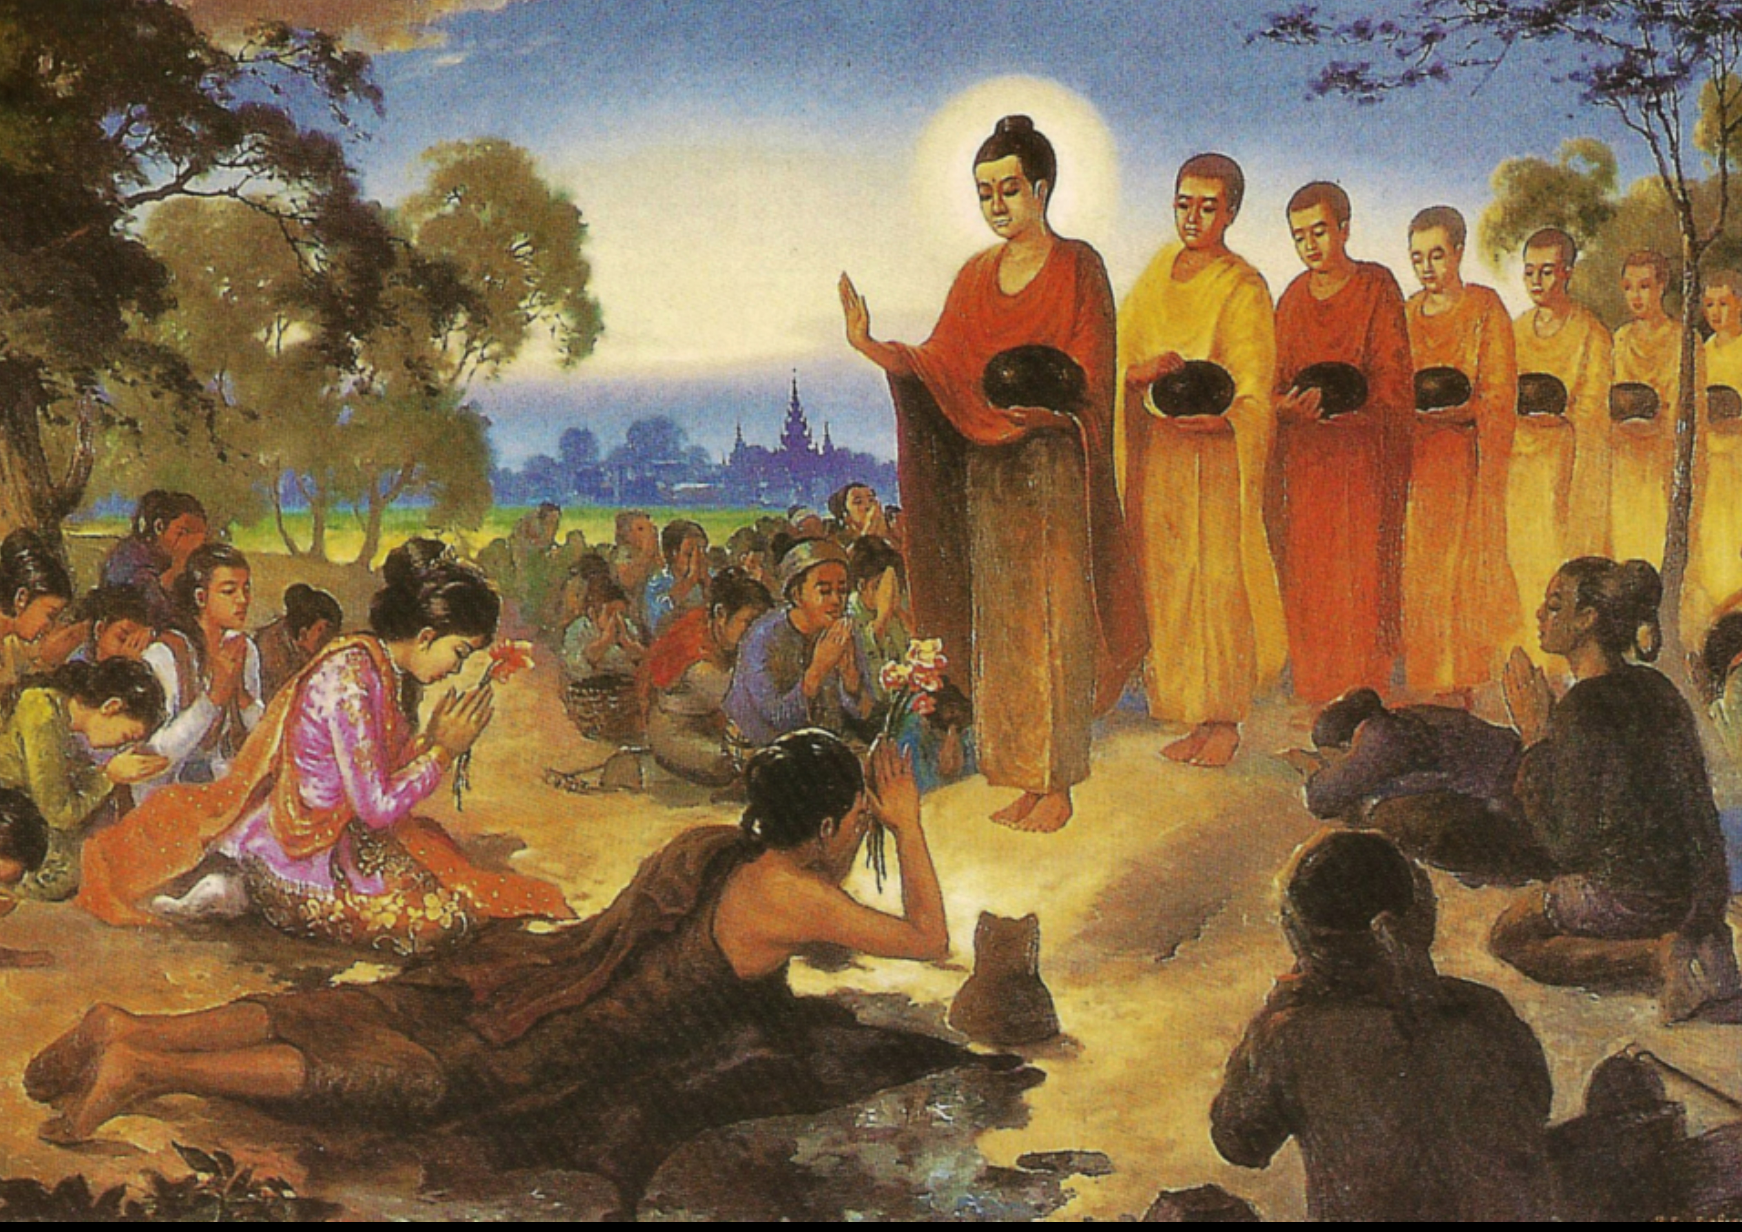
\includegraphics[width=300pt]{sumeda.png}
\end{frame}
\begin{frame}
\begin{itemize}
 \item Little chariot - DYOR; avoid medical interventions with more risk than benefit. Go to MedFree events, travel to where individual rights are more respected.\pause
 \item Big chariot - make ``The system'' work for benefit of the collective wellfare of the people.\emph{imo: very hard to do...maybe impossible?}
\end{itemize}

\end{frame}
\begin{frame}
 \frametitle{The great divide - as I see it}
 \begin{itemize}
  \item \textbf{One group}  - follows the rules, is mad at the other group for being selfish and not willing to sacrifice for the 
  social good.\pause
  \item \textbf{Second group} - doesn't believe the rules are for the social good.\pause
 \end{itemize}
%anecdotes - Asaf in store.
\textit{My view: Our cooperation and governance technologies are extremely primitive...can we do better?}\nl
\textit{One answer I like:Futarchy and Democracy DAOs}

\end{frame}

\begin{frame}
 \stitle{Before talking about futarchy - good time for break}
\end{frame}
\begin{frame}
 \frametitle{Prediction Markets}
 \begin{itemize}
  \item Bank sells for 1\$ pairs of bonds ($A$,$B$), e.g. signifying two candidates in an election.\pause
  \item After elections bank buys back bond of winning candidate for $1\$ $.\pause
  \item During election people trade these two bond types  on the free market - their price gives a prediction of 
  election result from people with \emph{skin in the game}
 \end{itemize}

\end{frame}
\begin{frame}
 \frametitle{Democracy DAO - Merkle (over simplified)}
 \textcolor{blue}{Instead of voting for a candidate or bill (e.g. brexit), people vote once a year by
 a number from zero to one saying ``How good was my last year''.}\nlnp
 $ACW_i\defeq$ the average of these numbers in year $i$. It's the Annual Collective Wellfare.
\end{frame}
\begin{frame}
 \frametitle{Prediction markets based on $ACW$}
 \begin{itemize}
  \item In beginning of year, bank sells for 1\$ pairs of bonds $(P,N)$. 
  \item At end of year bank redeems a $P$ for $ACW$ dollars and $N$ for $1-ACW$ dollars.
 \end{itemize}
 
\end{frame}
\begin{frame}
 \frametitle{Conditional Prediction markets}
\begin{itemize}
 \item We have a future event $E$, e.g. $E=$ ``brexit bill will pass''.\pause
 \item Bank sells for 1\$ a pair of bonds $(P_E,N_E)$.\pause
 \item If $E$ didn't happen, bank reimburses a dollar to buyers of bond pairs.\pause
 \item IF $E$ did happen - as before bank redeems $P_E$ for $ACW$ dollars and $N_E$ for $1-ACW$ dollars.
\end{itemize}
\end{frame}
\begin{frame}
 \frametitle{Governing in democracy DAO/futarchy}
 \begin{itemize}
  \item Given proposed law $L$, we start two conditional prediction markets - one with event $E=$``L was passed'',
  the other with event $F=$``L didn't pass''.\pause
  \item If after a while $P_E$ is worth more on the market than $P_F$, we pass the law; otherwise we don't.
 \end{itemize}

\end{frame}

\end{document}
